\footnotesize
\begin{tikzpicture}
\begin{axis}[
width=7cm,height=7cm,
axis x line=middle,
axis y line=middle,
axis equal,
xlabel=$\dfrac{V^*_{sf}}{\phi{}V_{sf}}$,
ylabel=$\dfrac{N^*_{tf}}{\phi{}N_{ti}}$,
x label style={at={(axis description cs:0.5,-0.05)},anchor=north},
y label style={at={(axis description cs:-0.15,.5)},anchor=south},
xmin=-.1,
ymin=-.1,
xmax=1.1,
ymax=1.1,
]
\addplot[domain=0:1,samples=2,line width=.8mm]({x},{1-x});
\end{axis}
\end{tikzpicture}